\documentclass{beamer}
\usepackage{ngerman}
% \usepackage{beamerthemelgdv}
\usepackage{./lgdv/beamerthemetest}
\usepackage[T1]{fontenc}
\usepackage[utf8]{inputenc}
\usepackage{subfigure}
\usepackage{listings}

% rough template

\title{Voxel Cone Tracing}
\subtitle{Graphics Project}
\author{Team 2\\P. Kögel, B. Mattes, J. Dörntlein}
\date{\today}

\newcommand{\TODO}[1]{{\large\bf Todo: #1}}

\subject{GraPro}	% goes to pdf meta
\keywords{Computer Graphics, Slides created with LaTeX}	% dito

\begin{document}

\frame{\titlepage}

% \usebackgroundtemplate{}
\newcommand{\slide}[2]{\frame{\frametitle{#1} #2}}
\newcommand{\topic}[1]{\frame{\begin{center}\huge\rm\textbf{#1}\end{center}}}

\slide{Overview}{
    \textbf{``Interactive indirect illumination using voxel cone tracing''}
	\begin{itemize}
        \item global illumination approach for game engines in realtime
        \item fast approximation through voxelization
        \item rays are bundled to cones -- intersection test with scene voxels
	\end{itemize}

    \begin{figure}[h]
    \centering
    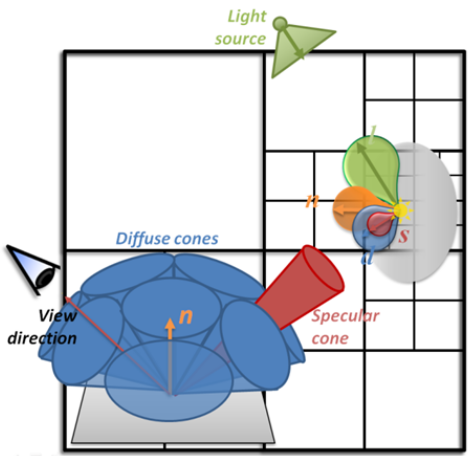
\includegraphics[width=150px]{img/voxel.png}
    %\caption{Voxel Cone Tracing.}
    \end{figure}
}

\slide{Voxelization}{
    % explain voxelization
}

\slide{Octree}{
    % explain the tree
}

\slide{Compositing}{
    \begin{itemize}
        \item ambient occlusion
        \item indirect diffuse phong
        \item indirect specular phong
    \end{itemize}

    % maybe point out some realworld examples like
    % cryengine or unrealengine
}

\slide{Live Demonstration}{
    % some example screenshots here
}

\end{document}

% vim: set foldmethod=marker foldmarker=[[[,]]]: 


